%%%%%%%%%%%%%%%%%%%%%%%%%%%%%%%%%%%%%%%%%%
%                                        %
% Szablon pracy dyplomowej inzynierskiej % 
%                                        %
%%%%%%%%%%%%%%%%%%%%%%%%%%%%%%%%%%%%%%%%%%



\documentclass[a4paper,twoside,12pt]{book}
\usepackage[utf8]{inputenc}                                      
\usepackage[T1]{fontenc}  
\usepackage{amsmath,amsfonts,amssymb,amsthm}
\usepackage[british,polish]{babel} 
\usepackage{indentfirst}
\usepackage{lmodern}
\usepackage{graphicx} 
\usepackage[hidelinks]{hyperref}
\usepackage{booktabs}
%\usepackage{tikz}
%\usepackage{pgfplots}
\usepackage{mathtools}
\usepackage{geometry}
\usepackage{amsmath}
\usepackage[page]{appendix} % toc,
\renewcommand{\appendixtocname}{Dodatki}
\renewcommand{\appendixpagename}{Dodatki}
\renewcommand{\appendixname}{Dodatek}

\usepackage{xcolor}

\usepackage{graphicx}
\usepackage{float}
\graphicspath{{./images/}}

\usepackage{setspace}
\onehalfspacing

\usepackage{dirtree}
\usepackage{hyperref}

\frenchspacing

\usepackage{listings}
%\lstset{
%	language={},
%	basicstyle=\ttfamily,
%	keywordstyle=\lst@ifdisplaystyle\color{blue}\fi,
%	commentstyle=\color{gray}
%}

%%%%%%%%%%%%%%%%%%%%%%%%%%%
% listingi 
% \usepackage{listings}
% \lstset{%
% 	language=python,%
% 	commentstyle=\textit,%
% 	identifierstyle=\textsf,%
% 	keywordstyle=\sffamily\bfseries, %\texttt, %
% 	%captionpos=b,%
% 	tabsize=3,%
% 	frame=lines,%
% 	numbers=left,%
% 	numberstyle=\tiny,%
% 	numbersep=5pt,%
% 	breaklines=true,%
% 	morekeywords={descriptor_gaussian,descriptor,partition,fcm_possibilistic,dataset,my_exception,exception,std,vector},%
% 	escapeinside={@*}{*@},%
% 	%texcl=true, % wylacza tryb verbatim w komentarzach jednolinijkowych
% }

\definecolor{codegreen}{rgb}{0,0.6,0}
\definecolor{codegray}{rgb}{0.5,0.5,0.5}
\definecolor{codepurple}{rgb}{0.58,0,0.82}
\definecolor{backcolour}{rgb}{0.95,0.95,0.92}

\lstdefinestyle{mystyle}{
    backgroundcolor=\color{backcolour},   
    commentstyle=\color{codegreen},
    keywordstyle=\color{magenta},
    numberstyle=\tiny\color{codegray},
    stringstyle=\color{codepurple},
    basicstyle=\ttfamily\footnotesize,
    breakatwhitespace=false,         
    breaklines=true,                 
    captionpos=b,                    
    keepspaces=true,                 
    numbers=left,                    
    numbersep=5pt,                  
    showspaces=false,                
    showstringspaces=false,
    showtabs=false,                  
    tabsize=2
}

\lstset{style=mystyle}

\lstset{%
	language=bash,%
	commentstyle=\textit,%
}
%%%%%%%%%%%%%%%%%%%%%%%%%%%%%%%%%%%%


%%%%%%%%%

%%%% TODO LIST GENERATOR %%%%%%%%%

%\usepackage{tikz}
%\usepackage{manfnt}   % dangerous sign 
\usepackage{color}
\definecolor{brickred}      {cmyk}{0   , 0.89, 0.94, 0.28}

\makeatletter \newcommand \kslistofremarks{\section*{Uwagi} \@starttoc{rks}}
  \newcommand\l@uwagas[2]
    {\par\noindent \textbf{#2:} %\parbox{10cm}
{#1}\par} \makeatother


\newcommand{\ksremark}[1]{%
{%\marginpar{\textdbend}
{\color{brickred}{[#1]}}}%
\addcontentsline{rks}{uwagas}{\protect{#1}}%
}

\newcommand{\comma}{\ksremark{przecinek}}
\newcommand{\nocomma}{\ksremark{bez przecinka}}
\newcommand{\styl}{\ksremark{styl}}
\newcommand{\ortografia}{\ksremark{ortografia}}
\newcommand{\fleksja}{\ksremark{fleksja}}
\newcommand{\pauza}{\ksremark{pauza `--', nie dywiz `-'}}
\newcommand{\kolokwializm}{\ksremark{kolokwializm}}

%%%%%%%%%%%%%% END OF TODO LIST GENERATOR %%%%%%%%%%%

%%%%%%%%%%%% ZYWA PAGINA %%%%%%%%%%%%%%%
% brak kapitalizacji zywej paginy
\usepackage{fancyhdr}
\pagestyle{fancy}
\fancyhf{}
\fancyhead[LO]{\nouppercase{\it\rightmark}}
\fancyhead[RE]{\nouppercase{\it\leftmark}}
\fancyhead[LE,RO]{\it\thepage}


\fancypagestyle{tylkoNumeryStron}{%
   \fancyhf{} 
   \fancyhead[LE,RO]{\it\thepage}
}

\fancypagestyle{NumeryStronNazwyRozdzialow}{%
   \fancyhf{} 
   \fancyhead[LO]{\nouppercase{\it\rightmark}}
   \fancyhead[RE]{\nouppercase{\it\leftmark}}
   \fancyhead[LE,RO]{\it\thepage}
}


%%%%%%%%%%%%% OBCE WTRETY  
\newcommand{\obcy}[1]{\emph{#1}}
\newcommand{\ang}[1]{{\selectlanguage{british}\obcy{#1}}}
%%%%%%%%%%%%%%%%%%%%%%%%%%%%%

% polskie oznaczenia funkcji matematycznych
\renewcommand{\tan}{\operatorname {tg}}
\renewcommand{\log}{\operatorname {lg}}

% jeszcze jakies drobiazgi

\newcounter{stronyPozaNumeracja}

\newcommand{\hcancel}[1]{%
    \tikz[baseline=(tocancel.base)]{
        \node[inner sep=0pt,outer sep=0pt] (tocancel) {#1};
        \draw[red] (tocancel.south west) -- (tocancel.north east);
    }%
}%

\newcommand{\miesiac}{%
  \ifcase\the\month
  \or styczeń% 1
  \or luty% 2
  \or marzec% 3
  \or kwiecień% 4
  \or maj% 5
  \or czerwiec% 6
  \or lipiec% 7
  \or sierpień% 8
  \or wrzesień% 9
  \or październik% 10
  \or listopad% 11
  \or grudzień% 12
  \fi}


%%%%%%%%%%%%%%%%%%%%%%%%%%%%%%%%%%%%%%%%%%%%%%
% Helvetica font macros for the title page:
\newcommand{\headerfont}{\fontfamily{phv}\fontsize{18}{18}\bfseries\scshape\selectfont}
\newcommand{\titlefont}{\fontfamily{phv}\fontsize{18}{18}\selectfont}
\newcommand{\otherfont}{\fontfamily{phv}\fontsize{14}{14}\selectfont}

\newcommand{\autor}{Szymon Ciemała}
\newcommand{\promotor}{dr inż. Krzysztof Jaskot}
\newcommand{\konsultant}{dr inż. Imię Nazwisko}
\newcommand{\tytul}{Tytuł pracy dyplomowej inżynierskiej}
\newcommand{\polsl}{Politechnika Śląska}
\newcommand{\wydzial}{Wydział Automatyki, Elektroniki i Informatyki}
\newcommand{\kierunek}{Kierunek: Automatyka i Robotyka}


\begin{document}
%\kslistofremarks 
%%%%%%%%%%%%%%%%%%%%%%%%%%%%%%%%%%%%%%%%%%%%%%%%%%%%%%%
%%%%%%%%%%%%%%%%%%  STRONA TYTULOWA %%%%%%%%%%%%%%%%%%%
%%%%%%%%%%%%%%%%%%%%%%%%%%%%%%%%%%%%%%%%%%%%%%%%%%%%%%%
\pagestyle{empty}
{
	\newgeometry{top=2.5cm,%
	             bottom=2.5cm,%
	             left=3cm,
	             right=2.5cm}
	\sffamily
	\rule{0cm}{0cm}
	
	\begin{center}
	
\includegraphics[width=29mm]{logo_pl.jpg}
	\end{center} 
	\vspace{1cm}
	\begin{center}
	\headerfont \polsl
	\end{center}
	\begin{center}
	\headerfont \wydzial
	\end{center}
	\begin{center}
	\headerfont \kierunek
	\end{center}
	\vfill
	\begin{center}
	\titlefont Praca dyplomowa inżynierska
	\end{center}
	\vfill
	
	\begin{center}
	\otherfont \tytul\par
	\end{center}
	
	\vfill
	
	\vfill
	 
	\noindent\vbox
	{
		\hbox{\otherfont autor: \autor}
		\vspace{12pt}
		\hbox{\otherfont kierujący pracą: \promotor}
		\vspace{12pt}  % zakomentuj, jezeli nie ma konsultanta
		\hbox{\otherfont konsultant: \konsultant} % zakomentuj, jezeli nie ma konsultanta
	}
	\vfill 
 
   \begin{center}
   \otherfont Gliwice,  \miesiac\ \the\year
   \end{center}	
	\restoregeometry
}
  

%\cleardoublepage
 

\rmfamily
\normalfont

%%%%%%%%%%%%%%%%%%%%%%%%%%%%%%%%%%%%%%%%%%%%%%%%%%%%%%%
%%%%%%%%%%%%%%%%%%%% SPIS TRESCI %%%%%%%%%%%%%%%%%%%%%%
%%%%%%%%%%%%%%%%%%%%%%%%%%%%%%%%%%%%%%%%%%%%%%%%%%%%%%%
\pagenumbering{Roman}
\pagestyle{tylkoNumeryStron}
\tableofcontents

%%%%%%%%%%%%%%%%%%%%%%%%%%%%%%%%%%%%%%%%%%%%%%%%%%%%%
\setcounter{stronyPozaNumeracja}{\value{page}}
\mainmatter
\pagestyle{empty}

%%%%%%%%%%%%%%%%%%%%%%%%%%%%%%%%%%%%%%%%%%%%%%%%%%%%%%%
%%%%%%%%%%%%%%%%%%% Streszczenie %%%%%%%%%%%%%%%%%%%%%%
%%%%%%%%%%%%%%%%%%%%%%%%%%%%%%%%%%%%%%%%%%%%%%%%%%%%%%%

\chapter{Streszczenie}

% Streszczenie pracy -odpowiednie pole w systemie APD powinno zawierac kopie tego streszczenia. Streszczenie, wraz ze slowami kluczowymi, nie powinno przekroczyc jednej strony.
%{\bf Slowa kluczowe:} 2-5 slow (fraz) kluczowych, oddzielonych przecinkami

%%Faktyczne streszczenie

\quad Praca inżynierska "Rozpoznawanie obiektów z wykorzystaniem biblioteki OpenCV", łączy tematykę wizji komputerowej oraz algorytmów uczenia maszynowego. 

\quad Praca skupia się na stworzeniu wygodnej w użyciu oraz powszechnie dostępnej biblioteki umożliwiającej wykorzystanie gestów oraz pozycji dłoni w dowolnych projektach napisanych w języku Python. 

\quad Do napisania pracy wykorzystano biblioteki języka Python o otwartym kodzie źródłowym, głównie OpenCV, MediaPipe oraz SciKit Learn. 

\addcontentsline{toc}{chapter}{Streszczenie}

%\cleardoublepage

\pagestyle{NumeryStronNazwyRozdzialow}

%%%%%%%%%%%%%% wlasciwa tresc pracy %%%%%%%%%%%%%%%%%

%%%%%%%%%%%%%%%%%%%%%% Wstęp %%%%%%%%%%%%%%%%%%%%%%%%

\chapter{Wstęp}
\begin{itemize}
\item wprowadzenie w problem/zagadnienie
\item osadzenie problemu w dziedzinie
\item cel pracy
\item zakres pracy
\item zwięzła charakterystyka rozdziałów
\item jednoznaczne określenie wkładu autora, w przypadku prac wieloosobowych – tabela z autorstwem poszczególnych elementów pracy
\end{itemize}

\newpage

\section{Wprowawdzenie w problem}
\quad Rozwój technolgii w ostatnich czasach przyczynił się do coraz częstszego wykorzystywania wizji komputerowej oraz metod uczenia maszynowego do rozpoznawania oraz klasyfikacji różnego typu obiektów, w tym części ludzkiego ciała. Pozwala to na interakcję człowieka z aplikacjami, często w spób bardziej naturalny. 

\section{Cel pracy}
Projekt inżynierski ma na celu stworzenie biblioteki w języku Python, która pozwoli na przystępne wykorzystanie algorytmów rozpoznawania gestów oraz ruchu dłoni. Biblioteka powinna oferować gotowe rozwiązania, na przykład przygotowane modele matematyczne pozwalające na rozpoznawanie języka migowego oraz gestów podstawowych. Dodatkowo powinna pozowlić na wyznaczenie pozycji dłoni, jej typu oraz wartości charakterystycznych, na przykład odlgłości między końcówkami wybranych palców czy kąta obrotu dłoni. 

\section{Osadzenie problemu w dziedzienie}
\quad Aktualnie istnieją częściowo gotowe rozwiązania pozwalające na rozpoznanie i klasyfikację dłoni - bibliotka MediaPipe. 

\section {Charakterystyka rozdziałów}

\quad W pierwszym rozdziale zostanie poruszony temat genezy problemu oraz jego sformułowania. Zostaną dodatkowo opisane jego założenia wraz z wyamaganą funkcjonalnością projektu. 

\quad W drugim temacie zostaną opisne techniczne tworzonej biblioteki oraz narzędzia wymagane do jej stworzenia. Zakres opisywanych narzędzi rozpocznie się od opisu wybranego systemu operacyjnego do programów służących do stworzenia pobieralnej paczki na platformi PyPi.

\quad W rozdziale nr 5 zostaną opisane wymagania sprzętowe wymagane do poprawnego działania funkcji biblioteki. Przedstawione zostanie działanie klasy wraz z jej parametrami oraz sposób jego wykorzysania. W drugiej jego części zostaną przedstawione przykłady wykorzysania modułu. Przykładowym projektami będą: program rozpoznający gest, interaktywny kiosk bezdotykowy i system doboru koloru przy pomocy gestu. 

\quad Kolejny rozdział opisuje budowę klasy wraz z najważniejszymi algorytmami oraz strukturami danych. Dodakowo opisany zostanie Jupyter Notebook służący do generowania modeli uczenia maszynowego rozpoznających gest dłoni. 

% \section{Ogólnie}

% Praca przedstawia wykorzystanie bibliotek OpenCV, MediaPipe oraz metod 
% uczenia maszynowego bibliteki SciKit Learn do stworzenia modułu dla 
% języka Python, który umożliwi sterwowanie dowolnymi aplikacjami przy 
% użyciu gestów oraz ruchu dłońmi. 

% \section{Wykorzystane technologie}
% \subsection{OpenCV}
% Biblioteka, dzieki której można wykorzystać obraz z kamery oraz wstępnie
% przetworzyć obraz, który zostanie wykorzystany przez bibliotekę MediaPipe.

% \subsection{MediaPipe}

% \quad
% Biblioteka MediaPipe o otwartym źródle, udostępnia wieloplatformowe oraz 
% konfigurowalne rozwiązania wykrzustujące uczenie maszynowe w dziedzienie 
% rozpoznawania, segmentacji oraz klasyfikacji obiektów wizji komputerowej. 
% Niektórymi z rozwiązań są:

% \begin{itemize}
%     \item Rozpoznawanie twarzy
%     \item Segmentacjia włosów oraz twarzy
%     \item Rozpoznawnie oraz określanie rozmiarów obiektów trójwymiarowych na podstawie obrazu dwuwymiarowego. 
% \end{itemize}

% Platformy/Języki programowania obsługiwane przez MediaPipe:

% \begin{itemize}
%     \item Android
%     \item IOS
%     \item JavaScript
%     \item Python
%     \item C++
%     \item Coral
% \end{itemize}

% ????
% Pozwoli na rozpoznaie dłoni oraz jej elementów charakterystycznych, 
% takich jak nagdarstek, stawy oraz końcówki palców. 
% ???


% \subsection{SciKit Learn}

% SciKit Learn to biblioteka, która oferuje różnego typu metody uczenia
% maszynowego. Biblioteka zawiera algorytmy klasyfikacji, regresjii oraz 
% analizy skupień. 
% Biblioteka pozwala na wykorzystanie metod klasyfikacji uczenia maszynowego. 
% Co pozwli na rozpoznanie gestów dłoni. 


%%%%%%%%%%%%%%%%%%%%% Analiza %%%%%%%%%%%%%%%%%%%%%%%

\chapter{Analiza Tematu}

% \begin{itemize}
% \item sformułowanie problemu
% \item osadzenie tematu w kontekście aktualnego stanu wiedzy ( state of the art ) o poruszanym problemie
% \item  studia literaturowe \cite{bib:artykul,bib:ksiazka,bib:konferencja,bib:url} -  opis znanych rozwiązań (także opisanych naukowo, jeżeli problem jest poruszany w publikacjach naukowych), algorytmów, 
% \end{itemize}


\section{Założenia}

\quad Wymagane możliwości oprogramowania można podzielić na trzy elementy:

\begin{itemize}
    \item Łatwość użytkowania
    \item Dostępność
    \item Możliwość dokładania własnych elementów
\end{itemize}

\quad Poprzez łatwość użytkowania można rozumieć oprogramowanie zapisane zgodnie z powszechnie stosowanymi standardami (\enquote{Zen of Python}) oraz przygotowaną dokumentację wraz z przykładami wykorzystania.  

\quad Paczka powinna być dostępna poprzez menedżer \textbf{pip}, dzięki czemu użytkownik ma możliwość instalacji z repozytorium paczki przy pomocy jednej komendy.

\quad Użytkownik powinien mieć możliwość stworzenia własnego modelu rozpoznającego gesty, na przykład przy pomocy interaktywnej instrukcji.

\section {Sformułowanie problemu}
% \quad Problem można podzielić na trzy części. Każda z nich odpowiada za wybraną część funkcjonalności biblioteki. 

% \begin{itemize}
%     \item Wyznaczenie pozyci dłoni, odległości pomiędzy wybranymi palcami oraz jej kąta obrotu. 
%     \item Rozpoznawanie gestów dłoni w dwóch trybach: prostym (parę dostępnych gestów) oraz zaawansowanym, który rozoznaje alfabet języka migowego. 
%     \item Dostępność biblioteki poprzez platfromę PyPi. 
% \end{itemize}

\quad Stworzenie modułu będzie wymagało napisania klasy pozwalającej na rozpoznanie elementów charakterystycznych dłoni oraz przetworzenia obrazu. Obraz będzie pochodził z kamerki internetowej, który zostanie odpowiednio przetworzony z wykorzystaniem funkcji dostępnych poprzez bibliotekę OpenCV. Przetworzony obraz zostanie wykorzystany przez metody biblioteki MediaPipe, która pozwoli na rozpoznanie elementów charakterystycznych dłoni. W napisanej klasie zostaną zaimplementowane metody, które pozwolą na rozpoznanie typu dłoni (prawa, lewa), odległości między paliczkiem palca wskazującego oraz kciuka, oraz obrotu dłoni. 

\quad Kolejnym elementem jest wygenerowanie modelu matematycznych klasyfikujących gesty dłoni. W tym celu zostanie wykorzystana biblioteka SciKit-Learn wraz z dostępnymi poprzez nią algorytmami ucznia maszynowego. Odpowiednio zebrane dane pozwolą na przeprowadzenie procesu ucznia dla kilku wybranych algorytmów. 

% \quad Najważniejszym elementem pracy jest powyżej wymieniony ostatni punkt listy. Dzięki wykorzystaniu platformy PyPi deweloperzy będą mogli przy pomocy programu \textbf{pip} za pomocą jednej komendy zainstalować paczkę wraz ze wszystkimi wymaganymi zależnościami. 

% \section{Podobne rozwiązania}

% \chapter{Założenia projektowe}

% \section{Budowa modułu}
% Moduł został napisany przy pomocy paradygmatu programowania
% obiektowego, co pozwala na przystępne wykorzystanie biblioteki w dowonych 
% projektach wymagających osbługi gestów. 

% \section{Dostęp}
% Całość projektu będzie dostępna na platformie GitHub wraz z możliwością 
% pobrania przy pomocy programu pip ze zdlanego repozytorium PyPi, dzięki czemu 
% pozowli to na sprawne i proste wykorzystanie modułu w dowolnym 
% projekcie. 

%%%%%%%%%%%%%%% Wymagania i Narzędia %%%%%%%%%%%%%%%%

\chapter{Wymagania i narzędzia}

% \begin{itemize}
% \item wymagania funkcjonalne i niefunkcjonalne
% \item przypadki użycia (diagramy UML) - dla prac, w których mają zastosowanie
% \item opis narzędzi, metod eksperymentalnych, metod modelowania itp.
% \item metodyka pracy nad projektowaniem i implementacją - dla prac, w których ma to zastosowanie
% \end{itemize}


\section{Wymagania funkcjonalne i niefunkcjonalne}

\quad Klasa powinna zawierać w sobie wszystkie niezbędne funkcje oraz parametry pozwalające na wykorzystanie jej w dowolnym projekcie, takie jak na przykład obliczanie kąta obrotu dłoni względem nadgarstka czy rozpoznawanie gestów. Dwa podstawowe modele rozpoznające gesty powinny zostać uprzednio przygotowane, natomiast użytkownik powinien mieć dodatkowo możliwość stworzenia własnego modelu rozpoznającego wybrane ułożenie dłoni. 

\quad Pobranie modułu powinno być możliwe poprzez wykorzystanie standardowego menedżera do zarządzania paczkami w języku Python, czyli programu \textbf{pip}. Ten menedżer pozwala na instalacje paczki wraz z jej zależnościami, czyli innymi paczkami wymaganiami do poprawnego działania pobieranej biblioteki. 

\quad Na głównej stronie projektu powinna zostać zamieszczona krótka dokumentacja w postaci pliku \textbf{README.md}, w którym zostanie opisany proces instalacji paczki, jej funkcjonalność oraz przykładowe programy. 

\section{Narzędzia}

\quad Przy tworzeniu modułu ważne są wykorzystywane narzędzia, zaczynając od wybranego systemu operacyjnego, a kończąc na programach pozwalających na przygotowanie plików źródłowych wysyłanych na zdalne repozytorium PyPi, każde z nich jest kluczowe do zbudowania pełnego projektu. 

\subsection{System operacyjny Ubuntu}
\quad Do stworzenia oprogramowania została wybrana dystrybucja Ubuntu w wersji 20.04 LTS. System został wybrany ze względu na istnienie takich elementów jak powłoka systemowa \textbf{bash}, menedżer pakietów oraz wsparcie dla języka Python. Główny powodem, dla którego ten system został wybrany, jest fakt istnienia rozbudowanej społeczność, która pomaga w rozwiązywaniu problemów. 

\subsection{GitHub}
\quad Platforma GitHub, która wykorzystuje rozproszony system kontroli Git, pozwala na stworzenie głównej strony biblioteki, na której znajdą się pliki programu wraz z dokumentacją oraz instrukcją instalacji i korzystania. W czasie pracy nad modułem system Git pomaga w tworzeniu kopii zapasowych. Zważając na fakt, że biblioteka jest wolnoźródłowa, GitHub może posłużyć jako system, który pozwala na rozbudowywanie projektu przez innych użytkowników lub tworzenia własnej i niezależnej wersji tego oprogramowania. 

\subsection{Python}
\quad Do napisania biblioteki został wykorzystany język skryptowy Python. Dzięki swojej popularności oraz dostępności Python stał się językiem powszechnie stosowanym w pracy związanej z zagadnieniami uczenia maszynowego, analizy danych oraz przetwarzania obrazów. Na platformie PyPi można znaleźć wiele narzędzi pozwalających na pracę właśnie w tych dziedzinach, jak i również wielu innych. 

\quad Ze względu na swoją budowę, Python nie należy do najwydajniejszych języków. Python jest językiem interpretowanym, co oznacza, że jego program nie zostaje skompilowany do kodu maszynowego, a zostaje on zinterpretowany przez interpreter. Ma to jednak swoje zalety, skrypt można wykonywać w częściach, co pozwala na testowanie działania programu. Dzięki czemu łatwiej jest znajdować błędy i na bieżąco je likwidować. Potencjał tego w pełni wykorzystuje interaktywna powłoka iPython. 

\subsection{iPython}
\quad To interaktywna powłoka dla języka Python, która rozszerza jego działanie o introspekcję, czyli możliwość wykonywania poprzednich części programu. W praktyce oznacza to, że użytkownik ma możliwość wykonywania programu zawartego w komórkach w dowolnej kolejności, nawet jeśli oznacza to wykonywanie programu zapisanego w komórkach poprzedzających aktualną. 

\quad Dodatkowo iPython oferuje możliwość korzystania z komend wiersza poleceń. Pozwala to, na przykład na instalowanie modułów wewnątrz programu. 

\subsection{Jupyter Notebook}

\quad Do obsługi interaktywnej powłoki iPython, wykorzystany został Jupyter Notebook (\enquote{notatnik}), czyli webowy edytor, który został stworzony z myślą o pracy związanej z analizą danych oraz obliczeniami naukowymi. 

\quad Dodatkowym atutem jest fakt, że Jupyter Notebook pozwala na zapis tekstu w języku Markdown, czyli języku znaczników stosowanym do formatowania tekstu. Co pozwala na czytelny opis programu oraz wstawianie obrazów, jeśli są wymagane. Dodatkowo wszystkie wykresy generowane przez na przykład przez bibliotekę \textbf{matplotlib} będą wyświetlane na stałe pod komórką, w której został wykonany program. Pozwala to na stworzenie programu, który może służyć jednocześnie jako interaktywna instrukcja. 

\subsection{Visual Studio Code}

\quad Do stworzenia oprogramowania został wybrany edytor Visual Studio Code. Edytor jest programem o otwartym kodzie źródłowym i został stworzony przez korporację Microsoft. Aplikacja posiada wiele darmowych rozszerzeń, często tworzonych przez użytkowników edytora. To właśnie dzięki rozszerzeniom program pozwala na pracę z wieloma typami plików oraz języków programowania.  

\subsection{Python Package Index}
\quad Python Package Index, w skrócie PyPi, jest platformą, na której udostępniane są moduły dla języka Python. Aktualnie jest ona zarządzana przez fundację \enquote{Python Software Foundation}. Paczki pobierane są przy pomocy programu \textbf{pip}, standardowo instalowanego wraz z językiem Python, co oznacza, że PyPi jest oficjalnym repozytorium oprogramowania właśnie dla tego języka. 

\quad Każdy użytkownik, organizacja lub firma mają możliwość stworzenia swojej własnej paczki i udostępnienia jej na repozytorium wraz z krótką dokumentacją oraz instrukcją instalacji.

\subsection{Programy bdist\_wheel, sdist orz twine}
\quad Oba programy są niezbędne do przygotowania w pełni działającej paczki udostępnianej na repozytorium PyPi. Program \textbf{sdist} pozwala na stworzenie źródłowej dystrybucji, czyli w praktyce pliku typu \textbf{.zip}, \textbf{.tar} czy też \textbf{.gztar}, w których znajdują się wybrane pliki będące częścią biblioteki. 

\quad Kolejnym programem jest \textbf{bdist\_wheel}, który odpowiada za stworzenie paczki typu \textbf{WHEEL}, która pozwala na szybszą instalację niż w przypadku instalacji wykorzystującej pliki źródłowe. WHEEL pozwala na pominięcie etapu kompilacji, przez co kompilator nie jest wymagany na sprzęcie użytkownika. 

\quad Ostatnim program jest \textbf{twine}, który pozwala na załadowanie gotowej paczki na repozytorium wraz z autoryzacją poprzez HTTPS. Program wspiera różne typy paczek, w tym typ WHEEL. 

% %%%%%%%%%%%%%%%%%%%%%%%%%%%%%%%%%%%%%%%%%%%%%%%%%%%%%%%%%%%%%%%%%%%%
% %%%%%%%%%%%%%%%%%%%%%%%%%%%% BIBLIOTEKI %%%%%%%%%%%%%%%%%%%%%%%%%%%%
% %%%%%%%%%%%%%%%%%%%%%%%%%%%%%%%%%%%%%%%%%%%%%%%%%%%%%%%%%%%%%%%%%%%%


\section{Biblioteki}

\quad Biblioteki opisane w tej sekcji są bibliotekami o otwartym kodzie źródłowym. Pozwala to na wykorzystanie ich w projekcie bez opłacania lub łamania żadnych licencji. 

\subsection{OpenCV}

\quad OpenCV \cite{bib:opencv_book} \cite{bib:opencv} jest biblioteką, która zajmuje się wizją komputerową, w tym głównie przetwarzaniem obrazów w czasie rzeczywistym. Projekt został rozpoczęty przez firmę Intel w 2001 roku, a później był wspierany przez laboratorium Willow Garge, które jest odpowiedzialne za stworzenie systemu ROS. OpenCV wspiera wiele języków programowania: C++, C\#, Python, Java oraz JavaScript, co oznacza, że jest to biblioteka wieloplatformowa i znajduje ona zastosowanie w wielu aplikacjach oraz systemach. 

\subsection{MediaPipe}

\quad Biblioteka MediaPipe \cite{bib:mediapipe} \cite{bib:mediapipe_1}, która została stworzona przy wsparciu firmy Google, udostępnia wieloplatformowe oraz konfigurowalne rozwiązania wykorzystujące uczenie maszynowe w dziedzinie rozpoznawania, segmentacji oraz klasyfikacji obiektów wizji komputerowej. Niektórymi z rozwiązań są:

\begin{itemize}
    \item Segmentacja włosów oraz twarzy
    \item Śledzenie pozycji obiektów
    \item Rozpoznawanie dłoni
\end{itemize}

\quad Oprogramowanie tworzone przez MediaPipe jest wysoce zoptymalizowane, co pozwala na wykorzystanie go na urządzeniach codziennego użytku, smartfonach, czy komputerach osobistych. 

% \quad Model modułu MediaPipe pozwala na wyznaczenie pozycji 21 elementów charakterystycznych dłoni. Współrzędne X i Y są znomralizowane względem rozdzielczości obrazu kamery. Współrzędna X względem liczby pikseli w osi X, a współrzędna Y względem liczby pikseli w osi Y. Oś Z jest prostopadła do osi X i Y, z punktem początkowym w punkcie określającym pozycję nadgarstka. Współrzędna Z jest znormalizowana względem szerokości obrazu kamery, tak jak współrzędna X. 

\subsection{SciKit-Learn}

\quad SciKit-Learn \cite{bib:scikit} \cite{bib:scikit_basics} początkowo został stworzony jako dodatek do biblioteki SciPy jako projekt w ramach \textbf{Google Summer of Code} w roku 2007. Biblioteka oferuje różnego typu metody uczenia maszynowego, w tym algorytmy klasyfikacji, regresji oraz analizy skupień. Przykładowym algorytmami w bibliotece są:
\begin{itemize}
    \item Las losowy -- polegająca na konstruowaniu wielu drzew decyzyjnych w czasie uczenia. 
    \item Algorytm centroidów -- algorytm wykorzystywany w analizie skupień.
    \item Maszyna wektorów nośnych -- algorytm klasyfikujący, często wykorzystywany w procesie rozpoznawania obrazów. 
\end{itemize}

%%%%%%%%%%%%%% Specyfikacja Zewnętrzna %%%%%%%%%%%%%%

% \chapter{Część techniczna/praktyczna}

% \chapter{Wymagania i narzędzia}

\chapter{[Właściwy dla kierunku - np. Specyfikacja zewnętrzna]}
Jeśli to Specyfikacja zewnętrzna:
\begin{itemize}
\item  wymagania sprzętowe i programowe
\item  sposób instalacji
\item  sposób aktywacji
\item  kategorie użytkowników
\item  sposób obsługi
\item   administracja systemem
\item  kwestie bezpieczeństwa
\item  przykład działania
\item  scenariusze korzystania z systemu (ilustrowane zrzutami z ekranu lub generowanymi dokumentami)
\end{itemize}

\begin{figure}
\centering

\includegraphics[width=3cm]{logo_pl.jpg}
\caption{Podpis rysunku po rysunkiem.}
\label{fig:2}
\end{figure}

\section{Wymagania sprzętowe i programowe}

\section{Przykład działania}

%%%%%%%%%%%%%% Specyfikacja Wewnętrzna %%%%%%%%%%%%%%

\chapter{[Właściwy dla kierunku - np.Specyfikacja wewnętrzna]}
Jeśli to Specyfikacja wewnętrzna:
\begin{itemize}
\item przedstawienie idei
\item architektura systemu
\item opis struktur danych (i organizacji baz danych)
\item komponenty, moduły, biblioteki, przegląd ważniejszych klas (jeśli występują)
\item przegląd ważniejszych algorytmów (jeśli występują)
\item szczegóły implementacji wybranych fragmentów, zastosowane wzorce projektowe
\item diagramy UML
\end{itemize}


\begin{itemize}
    \item wymagania funkcjonalne i niefunkcjonalne
    \item przypadki użycia (diagramy UML) - dla prac, w których mają zastosowanie
    \item opis narzędzi, metod eksperymentalnych, metod modelowania itp.
    \item metodyka pracy nad projektowaniem i implementacją - dla prac, w których ma to zastosowanie
    \end{itemize}
    
    \section{Rozpoznawanie dłoni}
    
    \quad Pierwszym elementem projektu jest rozpoznanie dłoni poprzez wyznacznie pozycji elementów charakterystycznych. Pozycja każdego z tych elementów jest względna wedłgu pozycji nadgarstka. ????
    
    
    %%%%%%%%%%%%%%%%%%%%%%%%%%%%%%%%%%%%%%%%%%%%%%%%%%%%%%%%%%%%%%%%%%%%
    %%%%%%%%%%%%%%%%%%%%%%%%%%%%%% OPEN CV %%%%%%%%%%%%%%%%%%%%%%%%%%%%%
    %%%%%%%%%%%%%%%%%%%%%%%%%%%%%%%%%%%%%%%%%%%%%%%%%%%%%%%%%%%%%%%%%%%%
    \subsection{OpenCV - przygotowanie obrazu z kamery}
    
    \quad Poprawne działanie modelu MediaPipe wymaga odpowiedniego przygotowania obrazu kamery. Działanie kontrolerolera odbywa się poprzez główną metodę \textbf{main()}.
    
    Metoda \textbf{main()} jest główną funkcją, w której dokonywane są obliczenia oraz przeszktałcenia pozwalające na obliczenie obrotu dłonie, odległości między wybranymi palcami oraz na wykrycie gestu. 
    
    % \inputminted[firstline=51, lastline=52]{python}{../OpenLeap.py}
    
    \lstinputlisting[language=python, firstline=51, lastline=52]{../OpenLeap.py}
    
    \quad W pierwszym kroku tworzymy instancję klasy \textbf{VideoCapture} biblioteki \textbf{OpenCV}, która pozwoli na odczytywanie obrazu kamery. 
    
    \lstinputlisting[language=python, firstline=272, lastline=297]{../OpenLeap.py}
    
    % \inputminted[firstline=272, lastline=297]{python}{../OpenLeap.py}
    
    %%%%%%%%%%%%%%%%%%%%%%%%%%%%%%%%%%%%%%%%%%%%%%%%%%%%%%%%%%%%%%%%%%%%
    %%%%%%%%%%%%%%%%%%%%%%%%%%%% MEDIA PIPE %%%%%%%%%%%%%%%%%%%%%%%%%%%%
    %%%%%%%%%%%%%%%%%%%%%%%%%%%%%%%%%%%%%%%%%%%%%%%%%%%%%%%%%%%%%%%%%%%%
    
    \subsection{MediaPipe - Elementy charakterystyczne}
    
    \quad Biblioteka MediaPipe o otwartym źródle, udostępnia wieloplatformowe oraz konfigurowalne rozwiązania wykrzustujące uczenie maszynowe w dziedzienie rozpoznawania, segmentacji oraz klasyfikacji obiektów wizji komputerowej. Niektórymi z rozwiązań są:
    
    \begin{itemize}
        \item Rozpoznawanie twarzy
        \item Segmentacjia włosów oraz twarzy
        \item Rozpoznawnie oraz określanie rozmiarów obiektów trójwymiarowych 
              na podstawie obrazu dwuwymiarowego. 
    \end{itemize}
    
    \quad Model modułu MediaPipe pozwala na wyznaczenie pozycji 21 elementów charakterystycznych dłoni. Współrzędne X i Y są znomralizowane względem rozdzielczości obrazu kamery. Współrzędna X względem liczby pikseli w osi X, a współrzędna Y względem liczby pikseli w osi Y. Oś Z jest prostopadła do osi X i Y, z punktem początkowym w punkcie określającym pozycję nadgarstka. Współrzędna Z jest znormalizowana względem szerokości obrazu kamery, tak jak współrzędna X. 
    
    \begin{figure}[H]
    \begin{center}
        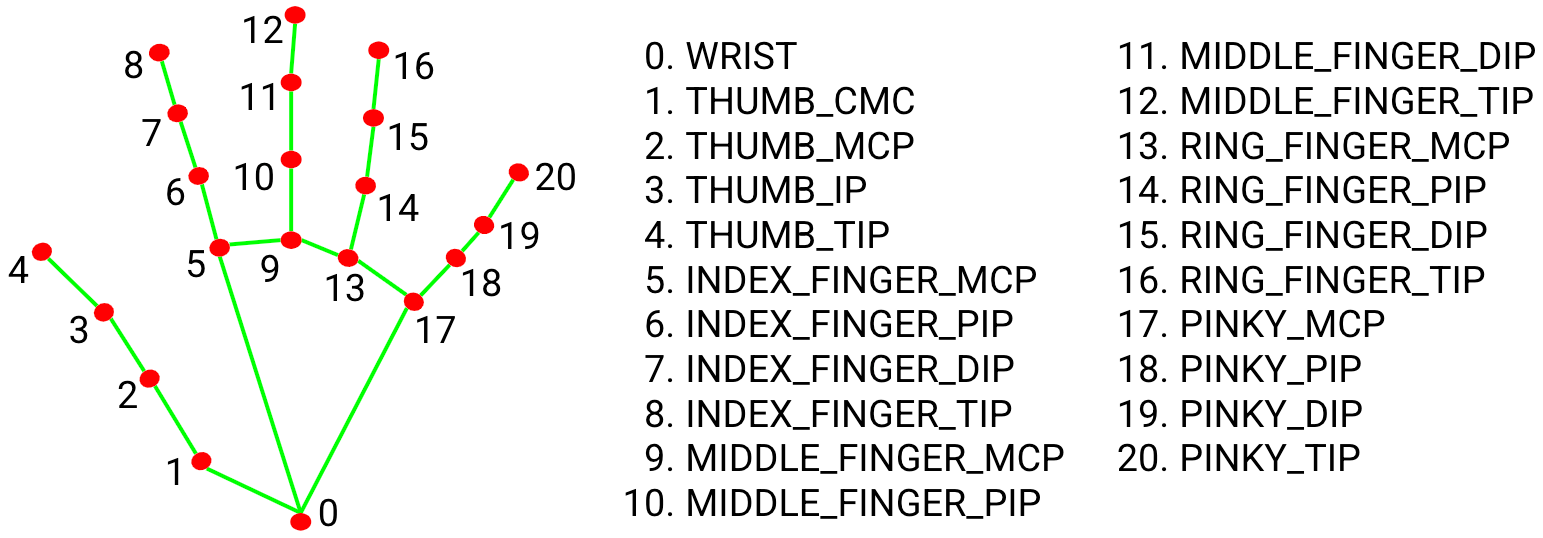
\includegraphics[width=15cm]{../images/hand_landmarks.png}
        \caption{Elementy charakterystyczne dłoni}
    \end{center}
    \end{figure}
    
    \quad Pozycje nadgarstka, paliczków oraz stawów dłoni zostaną wykorzystane do obliczenia obrotu dłoni względem punkut 0 oraz do wytrenowania modeli uczenia maszynowego, których zadaniem będzie rozpoznawnie wybranych gestów. 
    
    \subsection{Generowanie grafiki dłoni}
    
    \quad Generowanie grafiki nałożonej na daną dłoń wykonuje się przy pomocy przygotowanej funkcji biblioteki MediaPipe, która współpracuje z OpenCV. 
    
    %%%%%%%%%%%%%%%%%%%%%%%%%%%%%%%%%%%%%%%%%%%%%%%%%%%%%%%%%%%%%%%%%%%%
    %%%%%%%%%%%%%%%%%%%%%%%%%%% SciKit Learn %%%%%%%%%%%%%%%%%%%%%%%%%%%
    %%%%%%%%%%%%%%%%%%%%%%%%%%%%%%%%%%%%%%%%%%%%%%%%%%%%%%%%%%%%%%%%%%%%
    
    
    \section{SciKit Learn - uczenie maszynowe}
    
    \quad SciKit Learn to biblioteka, która oferuje różnego typu metody uczenia maszynowego. Biblioteka zawiera algorytmy klasyfikacji, regresjii oraz analizy skupień. Przykładowym algorytmami w bibliotece są:
    
    \begin{itemize}
        \item Las losowy - polegająca na konstruowaniu wielu drzew decyzyjnych w czasie uczenia. 
        \item Algorytm centroidów - algorytm wykorzystywany w analizie skupień.
        \item Maszyna wektorów nośnoych - algorytm klasyfikujący, często wykorzystywany w procesie rozpoznawania obrazów. 
    \end{itemize}
    
    O wszystkich dostępnych algorytmach informacje można znaleźć w ogólnodostępnej dokumentacji biblioteki. 
    
    
    
    \subsection{Budowa programu}
    Celem programu będzie stworzenie modeli matematycznych przy pomocy metod uczenia maszynowego, których celem będzie rozpoznawanie gestów dłoni. Proces tworzenie takiego modelu można podzielić na trzy kroki.
    
    \begin{itemize}
        \item Zebranie i przetworzenie danych. 
        \item Przygotowanie algorytmów klasyfikacji i znalezenie najdokładniejszego. 
        \item Zapis modelu do pliku typu \textbf{pickle}
    \end{itemize}
    
    \subsection{Zebranie danych}
    
    \quad Przygotowanie danych do przetworzenia będzie wymagało paru opercaji matematycznych. Współrzędne opisujące pozycje elementów charakterystycznych są znormalizowane względem wielkości obrazu pobranego z kamery, z czego wynika, że środek układu współrzęnych jest w prawym górnym rogu obrazu pobranego z kamery. W takim wypadku należy przprowadzić transformację, tutaj akurat przesunięcie układu współrzędnych do pozycji nadgarstka. Taka operacja pozwoli na pozbycie się uniezależnienie zmiennych od pozycji elementów dłoni na obrazie. Ostatecznie pozbywamy się pozycji nadarstka z wektora danych, ponieważ jest ona środkiem nowego układu współrzędnych. 
    
    \quad \textbf{Macierz przesunięcia}
    
    \begin{equation*}
        M_p = 
        \begin{bmatrix}
        1 & 0 & 0 & -x_0 \\
        0 & 1 & 0 & -y_0 \\
        0 & 0 & 1 & -z_0 \\
        0 & 0 & 0 & 1
        \end{bmatrix}
    \end{equation*}
    
    \quad Aby dane mogły zostać zinterpretowane przez algorytmy ucznenia maszynowego muszą one zostać przedstawione w postaci jednowymiarowej. Aktualna postać macierzy przedstawiającej wpółrzędne elementów charakterystycznych ma następującą postać. Indeksy współrzędnych są równoznaczne z indeksami elementów dłoni. 
    
    \begin{equation*}
        M_p = 
        \begin{bmatrix}
        x_1' & y_1' & z_1' \\
        x_2' & y_2' & z_2' \\
         & \vdots &     \\
        x_{21}' & y_{21}' & z_{21}'
        \end{bmatrix}
    \end{equation*}
    
    Dane w postaci jednowymiarowej mają postać następującego wektora. 
    
    \begin{equation*}
        A_f=
        \begin{bmatrix}
            x_1 & y_1 & z_1 & x_2 & y_2 & \cdots & y_{21} & z_{21}
        \end{bmatrix}
    \end{equation*}
    
    
    \quad Drugim krokiem jest uniezależnienie pozycji elementów od odległości dłoni od kamery. Najprostszym rozwiązaniem jest normalizacja wektora danych względem największej bezwzględnej wartości. 
    
    \quad \textbf{Normalizacja}
    
    % \begin{equation*}
    %     A_n=
        % \begin{bmatrix}
        %     x_1 & y_1 & z_1 & x_2 & y_2 & \cdots & y_{21} & z_{21}
        % \end{bmatrix}
    % \end{equation*}
    
    
    \begin{equation*}
        A_n=\dfrac{A_f}{max(abs(A_f))}
    \end{equation*}
    
    \quad Każdy nowy wektor zostaje zapisany do pliku CSV z odpwowiednią etykietą. Zebrane dane posłużą do wytrenowania algorytmów uczenia maszynowego. 
    
    
    
    \subsection{Metody klasyfikacji - uczenie maszynowe}
    
    \quad Przygotowane dane zostają odczytane z pliku CSV. W pierwszym kroku należy rozdzielić je na dwie części: współrzędne (dane wejściowe) oraz etykiety (dane wyjściowe). W kolejnym kroku należy te dwie grupy podzielić na grupę trenującą i grupę testową. Zadaniem grupy testowej będzie trenowanie wybranych modeli matematycznych, a grupy testowej przetestowanie ich dokładności. 
    
    \quad W celu wybrania najlepszej metody klasyfikacji, zostnie wybranych kilka algorytmów. Każdy z nich stworzy swój model, a ostatecznie zostanie sprawdzona ich poprawności z wykorzystaniem grupy testowej. Model z najepszym wynikiem zostanie zapisany do pliku typu \textbf{pickle}. W języku Python pliki typu \textbf{pickle} pozwalają na zapis zmiennych, obiektów lub innych struktur danych, które mają zostać wykorzystane w po zakończeniu programu. 
    
    \subsection{Ponowne wykorzystanie modelu}
    
    \quad Gotowy model pobieramy i testujemy w przykładowym programie. 
    
    \section{Paczka PyPi}
    \subsection{Budowa paczki}
    
    \quad Ostatecznym krokiem jest przygotowanie programu w formie paczki, która zostanie udostępniona na platformie PyPi. Wygama to przygotowania odpowiednich plików konfiguracyjnych oraz zostosowania stosownych narzędzi do stworznie pliku \textbf{wheel} oraz \textbf{tar}. 
    
    \subsection{Struktura Paczki}
    \quad Pierwszm krokiem jest przygotowanie odpowiedniej struktury paczki. Do tego celu został stworzony folder o poniższej strukturze. W tym folderze znajdują się wszystkie potrzebne elementy paczki. W podfolderze o tej samej nazwie znajduje się główna części modułu, czyli plik .py, w którym zapisana jest klasa OpenLeap. Dodatkowo w tym folderze znajdują się pliki typu \textbf{pickle}, w których zapisane są modele rozpoznające gesty.
    
    \begin{figure}
    \centering
        \begin{minipage}{7cm}
            \dirtree{%
            .1 openleap.
            .2 openleap.
            .3 \hyperref[openleap-file1]{\_\_init\_\_.py}.
            .3 \hyperref[openleap-file2]{OpenLeap.py}.
            .3 \hyperref[openleap-file3]{gesture\_recognition.pkl}.
            .3 \hyperref[openleap-file4]{sign\_language\_alphabet.pkl}.
            .2 LICENSE.
            .2 MANIFEST.
            .2 README.md.
            .2 setup.py.
            } 
        \end{minipage}
        \caption{Struktura paczki PyPi}
    \end{figure}
    
    \subsection{Pliki Konfiguracyjne}
    \quad Pliki setup.py oraz MANIFEST są plikami, które odpowiadają za konfigurację oraz opis paczki. W pliku setup.py zapisany jest numer aktualnej wersji, autor, kontakt do autora, nazwa paczki itp. 
    
    \quad 
    
    
    % \subsection{Plik setup.py}
    \subsection{Załadowanie paczki do repozytorium}
    
    \quad Przed załadowaniem paczki do repozytorium, należy stworzyć zapakowaną paczkę źródłową, na przykład typu .tar oraz plik typu WHEEL. Oba pliki spełniają tą samą funkcję, czyli przechowywnie niezbędnych elementów paczki oraz umożliwiają ich instalację na systemie użytkownika. Plik WHEEL pozwala na dużo szybszy proces instalacji niż instalacja ze źródła, czyli paczki typu .tar. 


%%%%%%%%%%%%%%% Weryfikacja i Walidacje %%%%%%%%%%%%%%%%
\chapter{Weryfikacja i walidacja}
\begin{itemize}
\item sposób testowania w ramach pracy (np. odniesienie do modelu V)
\item organizacja eksperymentów
\item przypadki testowe zakres testowania (pełny/niepełny)
\item wykryte i usunięte błędy
\item opcjonalnie wyniki badań eksperymentalnych
\end{itemize}

\begin{table}
\centering
\caption{Opis tabeli nad nią.}
\label{id:tab:wyniki}
\begin{tabular}{rrrrrrrr}
\toprule
	         &                                     \multicolumn{7}{c}{metoda}                                      \\
	         \cmidrule{2-8}
	         &         &         &        \multicolumn{3}{c}{alg. 3}        & \multicolumn{2}{c}{alg. 4, $\gamma = 2$} \\
	         \cmidrule(r){4-6}\cmidrule(r){7-8}
	$\zeta$ &     alg. 1 &   alg. 2 & $\alpha= 1.5$ & $\alpha= 2$ & $\alpha= 3$ &   $\beta = 0.1$  &   $\beta = -0.1$ \\
\midrule
	       0 &  8.3250 & 1.45305 &       7.5791 &    14.8517 &    20.0028 & 1.16396 &                       1.1365 \\
	       5 &  0.6111 & 2.27126 &       6.9952 &    13.8560 &    18.6064 & 1.18659 &                       1.1630 \\
	      10 & 11.6126 & 2.69218 &       6.2520 &    12.5202 &    16.8278 & 1.23180 &                       1.2045 \\
	      15 &  0.5665 & 2.95046 &       5.7753 &    11.4588 &    15.4837 & 1.25131 &                       1.2614 \\
	      20 & 15.8728 & 3.07225 &       5.3071 &    10.3935 &    13.8738 & 1.25307 &                       1.2217 \\
	      25 &  0.9791 & 3.19034 &       5.4575 &     9.9533 &    13.0721 & 1.27104 &                       1.2640 \\
	      30 &  2.0228 & 3.27474 &       5.7461 &     9.7164 &    12.2637 & 1.33404 &                       1.3209 \\
	      35 & 13.4210 & 3.36086 &       6.6735 &    10.0442 &    12.0270 & 1.35385 &                       1.3059 \\
	      40 & 13.2226 & 3.36420 &       7.7248 &    10.4495 &    12.0379 & 1.34919 &                       1.2768 \\
	      45 & 12.8445 & 3.47436 &       8.5539 &    10.8552 &    12.2773 & 1.42303 &                       1.4362 \\
	      50 & 12.9245 & 3.58228 &       9.2702 &    11.2183 &    12.3990 & 1.40922 &                       1.3724 \\
\bottomrule
\end{tabular}
\end{table}  
 

%%%%%%%%%%%%%%%%%% Podsumowanie %%%%%%%%%%%%%%%%%%%
\chapter{Podsumowanie i wnioski}
\begin{itemize}
\item uzyskane wyniki w świetle postawionych celów i zdefiniowanych wyżej wymagań
\item kierunki ewentualnych danych prac (rozbudowa funkcjonalna …)
\item problemy napotkane w trakcie pracy
\end{itemize}

 
\bibliographystyle{plplain}
\bibliography{bibliografia}
\addcontentsline{toc}{chapter}{Bibliografia}


\begin{appendices}
 

\chapter*{Spis skrótów i symboli}
\addcontentsline{toc}{chapter}{Spis skrótów i symboli}

\begin{itemize}
\item[DNA] kwas deoksyrybonukleinowy (ang. \ang{deoxyribonucleic acid})
\item[MVC] model -- widok -- kontroler (ang. \ang{model--view--controller}) 
\item[$N$] liczebność zbioru danych
\item[$\mu$] stopnień przyleżności do zbioru
\item[$\mathbb{E}$] zbiór krawędzi grafu
\item[$\mathcal{L}$] transformata Laplace'a 
\end{itemize}


\chapter*{Źródła}
\addcontentsline{toc}{chapter}{Źródła}

Jeżeli w pracy konieczne jest umieszczenie długich fragmentów kodu źródłowego, należy je przenieść do załącznika.


\chapter*{Zawartość dołączonej płyty}
\addcontentsline{toc}{chapter}{Zawartość dołączonej płyty}

Do pracy dołączona jest płyta CD z~następującą zawartością:
\begin{itemize}
\item praca (źródła \LaTeX owe i końcowa wersja w \texttt{pdf}),
\item źródła programu,
\item dane testowe.
\end{itemize}

\listoffigures
\listoftables
	
\end{appendices}


\end{document}


%% Finis coronat opus.
